%-----------------------------------LICENSE------------------------------------%
%   This file is part of tikz_figures.                                         %
%                                                                              %
%   tikz_figures is free software: you can redistribute it and/or              %
%   modify it it under the terms of the GNU General Public License as          %
%   published by the Free Software Foundation, either version 3 of the         %
%   License, or (at your option) any later version.                            %
%                                                                              %
%   tikz_figures is distributed in the hope that it will be useful,            %
%   but WITHOUT ANY WARRANTY; without even the implied warranty of             %
%   MERCHANTABILITY or FITNESS FOR A PARTICULAR PURPOSE.  See the              %
%   GNU General Public License for more details.                               %
%                                                                              %
%   You should have received a copy of the GNU General Public License along    %
%   with tikz_figures.  If not, see <https://www.gnu.org/licenses/>.           %
%------------------------------------------------------------------------------%

% Use the standalone class for displaying the tikz image on a small PDF.
\documentclass[crop, tikz]{standalone}

% Import the tikz package to use for the drawing.
\usepackage{tikz}

% Tikz libraries used in the drawing.
\usetikzlibrary{hobby}

% Begin the document.
\begin{document}

    % Draw the figure.
    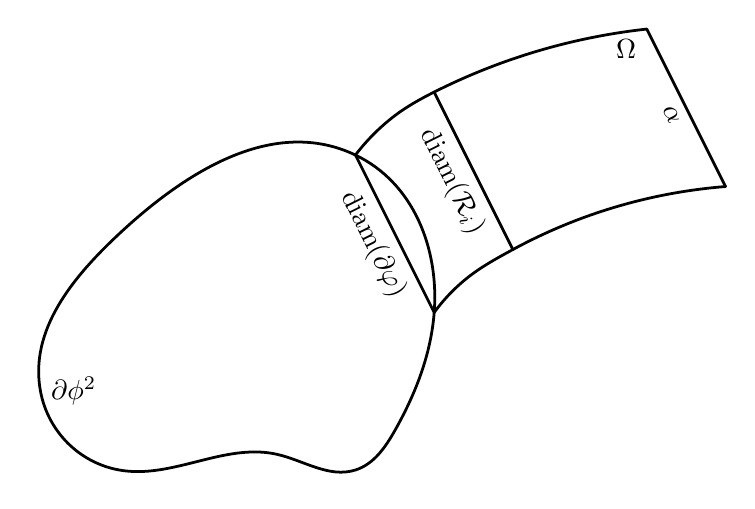
\begin{tikzpicture}[line width=1pt,line cap = round]

        % Positions of all of the points.
        \coordinate (a) at (0.0, 1.0);
        \coordinate (b) at (1.0, 3.0);
        \coordinate (c) at (4.0, 4.0);
        \coordinate (d) at (5.0, 2.0);
        \coordinate (e) at (4.5, 0.5);
        \coordinate (f) at (4.0, 0.0);
        \coordinate (g) at (3.0, 0.2);
        \coordinate (h) at (1.0, 0.0);
        \coordinate (i) at (4.5, 4.5);
        \coordinate (j) at (5.0, 4.8);
        \coordinate (k) at (7.7, 5.6);
        \coordinate (l) at (5.5, 2.5);
        \coordinate (m) at (6.0, 2.8);
        \coordinate (n) at (8.7, 3.6);

        % Label the two curves.
        \node at (a) [right] {$\partial\phi^{2}$};
        \node at (k) [below left] {$\Omega$};

        % Hobby curve for the blob curve.
        \path[%
            draw,
            use Hobby shortcut,
            closed = true
        ] (a) .. (b) .. (c) .. (d) .. (e) .. (f) .. (g) .. (h);

        % Draw the second blob.
        \draw (c) to [quick curve through = (i) .. (j)] (k);
        \draw (k) to node[midway, below, sloped] {$\alpha$} (n);
        \draw (n) to [quick curve through = (m) .. (l)] (d);
        \draw (m) to node[midway, below, sloped]
            {$\textrm{diam}(\mathcal{R}_i)$} (j);
        \draw (d) to node[midway, below, sloped]
            {$\textrm{diam}(\partial\varphi)$} (c);
    \end{tikzpicture}
\end{document}
